%% Dokumenteinstellungen %%%%%%%%%%%%%%%%%%%%%%%%%%%%%%%%%%%%
\documentclass[a4paper,oneside,12pt,ngerman]{scrartcl}

%% Deutsche Anpassungen %%%%%%%%%%%%%%%%%%%%%%%%%%%%%%%%%%%%%
\usepackage[ngerman]{babel}
\usepackage[T1]{fontenc}
\usepackage[ansinew]{inputenc}
\usepackage{lmodern} %Type1-Schriftart f�r nicht-englische Texte
\usepackage{booktabs}	% sch�nere tabellen

%% Packages f�r Grafiken & Abbildungen %%%%%%%%%%%%%%%%%%%%%%
\usepackage{graphicx} %%Zum Laden von Grafiken
%\usepackage{subfig} %%Teilabbildungen in einer Abbildung
%\usepackage{tikz} %%Vektorgrafiken aus LaTeX heraus erstellen


%% Packages f�r Formeln %%%%%%%%%%%%%%%%%%%%%%%%%%%%%%%%%%%%%
\usepackage{amsmath}
\usepackage{amsthm}
\usepackage{amsfonts}


%% Andere Packages %%%%%%%%%%%%%%%%%%%%%%%%%%%%%%%%%%%%%%%%%%
%\usepackage{a4wide} %%Kleinere Seitenr�nder = mehr Text pro Zeile.
\usepackage{fancyhdr} %%Fancy Kopf- und Fu�zeilen
%\usepackage{longtable} %%F�r Tabellen, die eine Seite �berschreiten
\usepackage{lastpage}
\usepackage[raggedright]{subfigure}
\usepackage[final]{pdfpages}
\includepdfset{pages=-,noautoscale}


%%%%%%%%%%%%%%%%%%%%%%%%%%%%%%%%%%%%%%%%%%%%%%%%%%%%%%%%%%%%%
%% Optionen / Modifikationen
%%%%%%%%%%%%%%%%%%%%%%%%%%%%%%%%%%%%%%%%%%%%%%%%%%%%%%%%%%%%%
%%%%%%%%%%%%%%%%%%%%%%%%%%%%%%%%%%%%%%%%%%%%%%%%%%%%%%%%%%%%%
%%                                                         %%
%%                     EINSTELLUNGEN                       %%
%%                                                         %%
%%%%%%%%%%%%%%%%%%%%%%%%%%%%%%%%%%%%%%%%%%%%%%%%%%%%%%%%%%%%%

%%%%%%%%%%%%%%%%%%%%%%%%%%%%%%%%%%%%%%%%%%%%%%%%%%%%%%%%%%%%%
%% HYPER REF
%%%%%%%%%%%%%%%%%%%%%%%%%%%%%%%%%%%%%%%%%%%%%%%%%%%%%%%%%%%%%
\usepackage[
hyperindex=true,
colorlinks=true,
linkcolor=black,
citecolor=black,
filecolor=black,
menucolor=black,
urlcolor=cyan,
breaklinks=true,
bookmarks=true,
bookmarksopen=false,
bookmarksnumbered=false,
pdfhighlight=/O,
]{hyperref}

%%%%%%%%%%%%%%%%%%%%%%%%%%%%%%%%%%%%%%%%%%%%%%%%%%%%%%%%%%%%%
%% FANCY HEADERS
%%%%%%%%%%%%%%%%%%%%%%%%%%%%%%%%%%%%%%%%%%%%%%%%%%%%%%%%%%%%%
% --- Kopf- und Fusszeilen - {} = rechts (gerade), [] = links (ungerade)
% letzte seite: \pageref{LastPage}
% doppelseitig:
%\lhead{Elektronik: \textbf{Oszilatorschaltungen}}	\chead{}		\rhead{Cyril Stoller und Hannes Stauffer}
%\lfoot{\today}	\cfoot{}		\rfoot{Seite \thepage\ von \pageref{LastPage}}

% einseitig:
%\lhead{\rightmark}			\chead{}					\rhead{}
%\lfoot{\leftmark}			\cfoot{}					\rfoot{Seite \thepage\ von \pageref{\LastPage}}

%\setlength{\headrulewidth}{0.4pt}
%\setlength{\footrulewidth}{0.4pt}


% Formeln r�misch nummerieren
\renewcommand{\theequation}{\Roman{equation}} 

% "Formel" statt "Gleichung"
\def\equationname{Formel}

%%%%%%%%%%%%%%%%%%%%%%%%%%%%%%%%%%%%%%%%%%%%%%%%%%%%%%%%%%%%%
%% DOKUMENT
%%%%%%%%%%%%%%%%%%%%%%%%%%%%%%%%%%%%%%%%%%%%%%%%%%%%%%%%%%%%%
\begin{document}

\title{Praktikum: DC-Motor}
\date{\today}
\author{Cyril Stoller, Marcel B�rtschi}
\maketitle

%% Inhaltsverzeichnis %%%%%%%%%%%%%%%%%%%%%%%%%%%%%%%%%%%%%%%
\tableofcontents %Inhaltsverzeichnis

\vfill

\listoffigures

%\pagestyle{fancy} %%Ab hier die Kopf-/Fusszeilen: headings / fancy / ...

\newpage
%
%\begin{abstract}
%	
%\begin{center}	
%\textbf{Abstract}
%\vspace{0.3cm}
%
%In diesem Versuch wird ein Gleichstrommotor und ein Gleichstromgenerator ausgemessen.
%\end{center}
%	
%\end{abstract}
%
%\vspace{2cm}


%%%%%%%%%%%%%%%%%%%%%%%%%%%%%%%%%%%%%%%%%%%%%%%%%%%%%%%%%%%%%
%%                                                         %%
%%         Kapitel / Hauptteil des Dokumentes              %%
%%                                                         %%
%%%%%%%%%%%%%%%%%%%%%%%%%%%%%%%%%%%%%%%%%%%%%%%%%%%%%%%%%%%%%



\section{Ziel}

Dieser Bericht beinhaltet genaue Angaben zur Durchf�hrung und eine Diskussion des Versuches \emph{Messversuch Gleichstrommaschine} im Mechatronik-Modul \emph{BTE5360}.

\section{Einleitung}

\subsection{Motivation}
Die in der Vorlesung erlernte Theorie soll mit diesem Praktikum in der Praxis nachvollzogen und vertieft werden. Anhand von zwei mechanisch gekoppelten Motoren wird das grundlegende elektrotechnische Verhalten eines DC-Motors als Motor und als Generator nachgewiesen und die im Unterricht behandelten Formeln auf reale Messwerte angewendet.

\subsection{Aufgabenstellung}
Die Aufgabenstellung ist unter \url{http://moodle.bfh.ch/} oder in \autoref{sec:aufgabe} zu finden.

\section{Durchf�hrung}
Hier werden nun die einzelnen Aufgaben separat und mit jeweils eigener abschliessender Diskussion behandelt. Im Folgenden wird der linke Motor auf dem Messaufbau \emph{Motor 1} und der rechte Motor \emph{Motor 2} genannt.

\begin{figure}[ht]
	\centering
		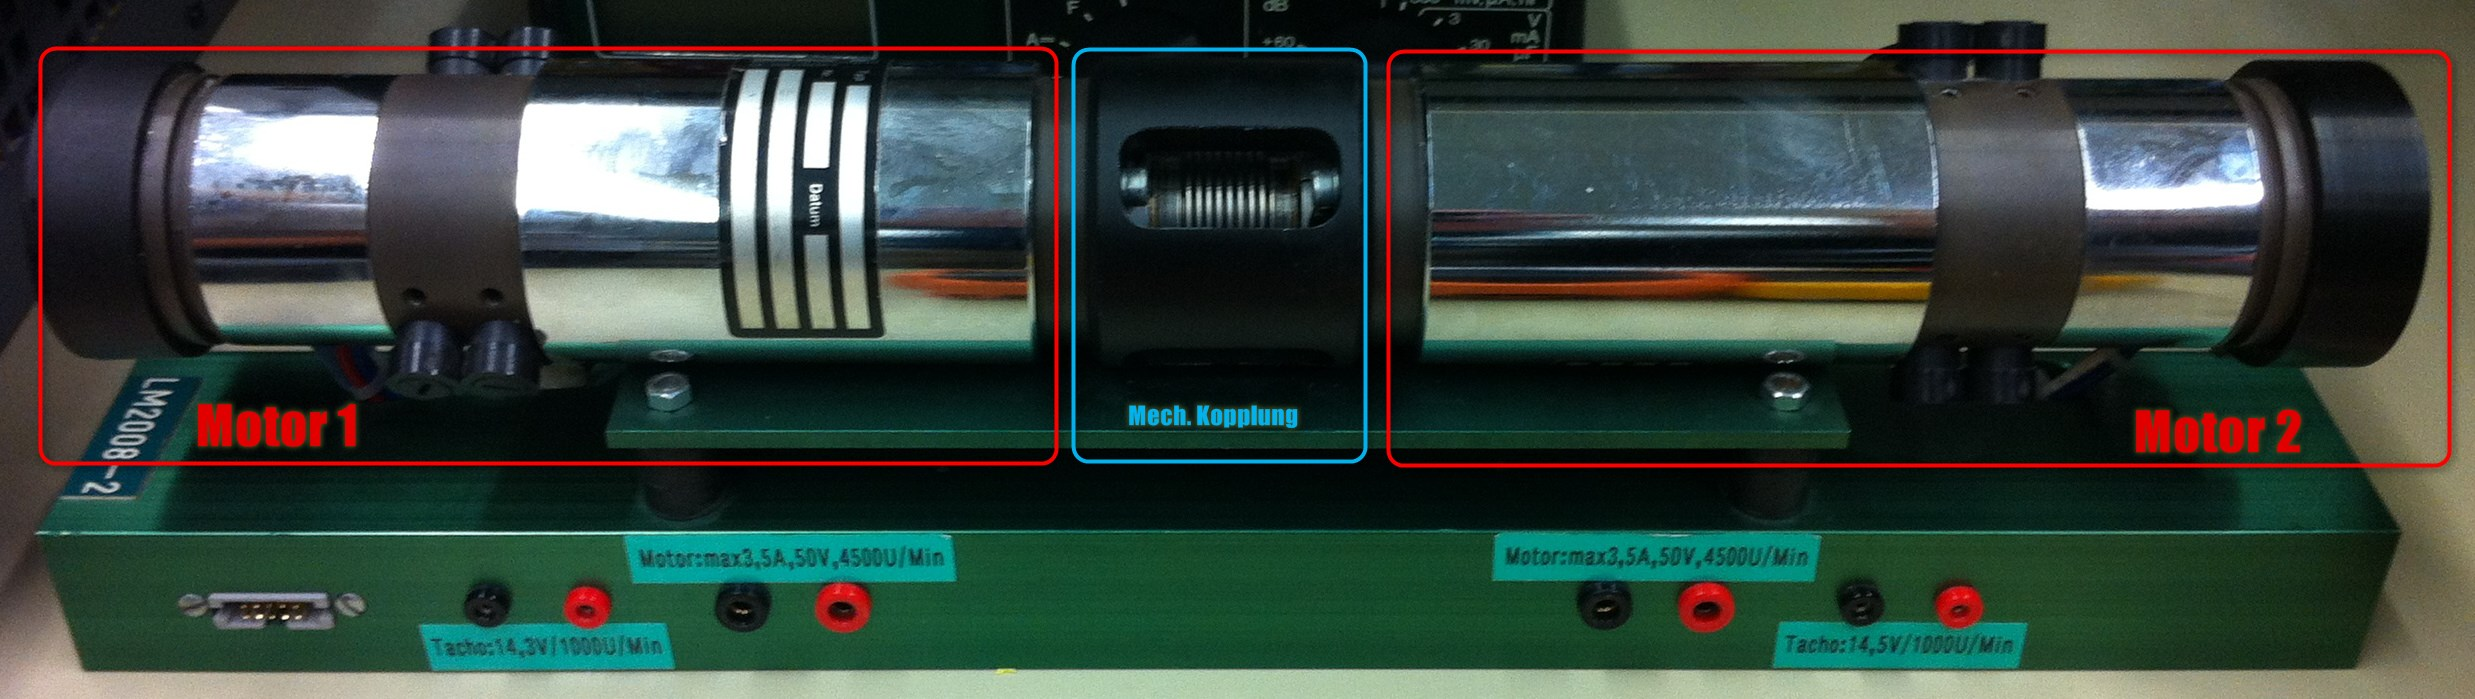
\includegraphics[width=1\textwidth]{images/AufbauModell.jpg}
	\caption{Aufbau Modell}
	\label{fig:AufbauModell}
\end{figure}

\subsection{Aufgabe 1}
Das Schema f�r die Aufgabe 4 ist in \autoref{fig:schema4} zusehen, das Schema f�r die Aufgaben 5, 7 und 8 in \autoref{fig:schema578}.

\begin{figure}[ht]
	\centering
		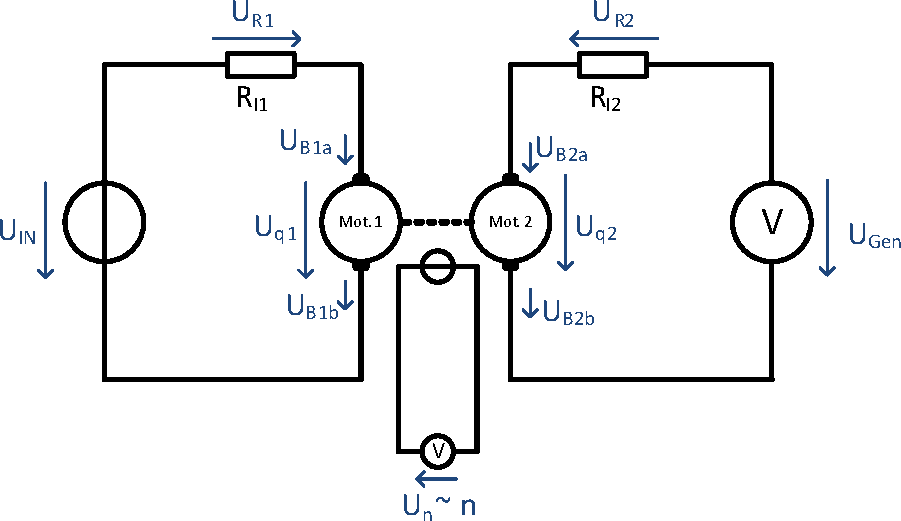
\includegraphics[width=0.6\textwidth]{images/SchemaAufg4.pdf}
	\caption{Messschema f�r Aufgabe 4}
	\label{fig:schema4}
\end{figure}

\begin{figure}[ht]
	\centering
		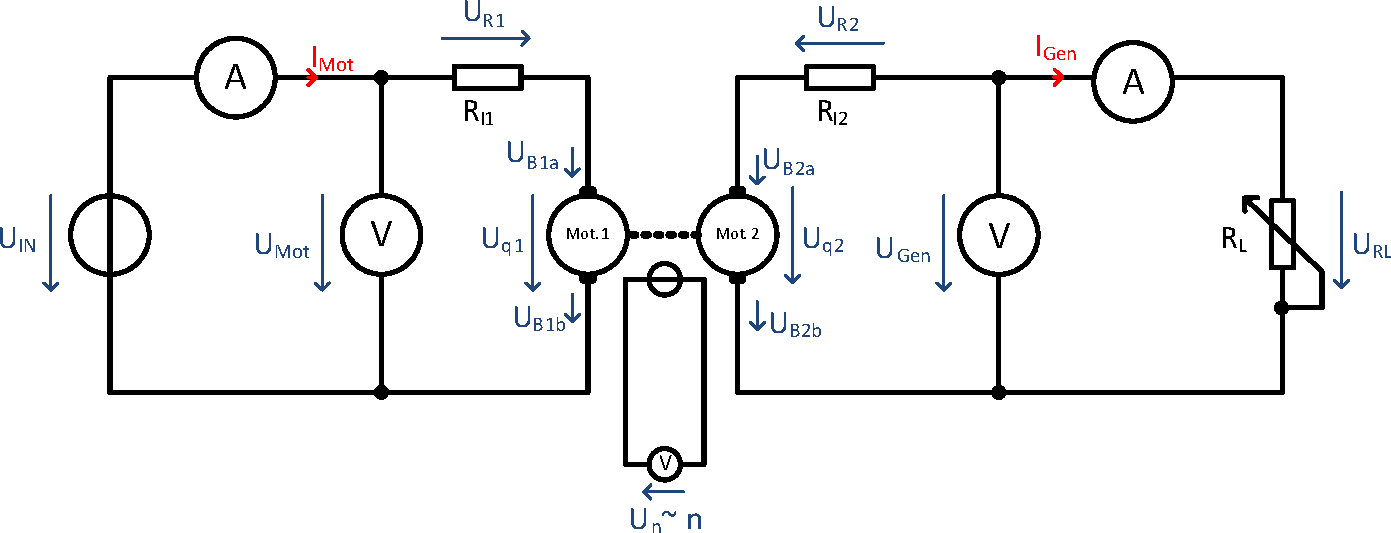
\includegraphics[width=0.8\textwidth]{images/SchemaAufg578.pdf}
	\caption{Messschema f�r die Aufgaben 5, 7 und 8}
	\label{fig:schema578}
\end{figure}

\subsection{Aufgabe 2}
Bei unterschiedlichen Rotorstellungen haben wir die Werte in \autoref{tab:widerstaende} gemessen.

\begin{table}[ht]\centering
\begin{tabular}{@{}llllll@{}}
	\toprule
	 & \multicolumn{4}{c}{Widerstandsmessungen [$\Omega$]} & Mittelwert [$\Omega$] \\
	\midrule
	Motor 1	&	3.3 & 2.7 & 3.0 & 3.6 & 3.15 \\
	Motor 2	& 2.4 & 2.7 & 2.9 & 3.2 & 2.8 \\
	\bottomrule
\end{tabular}
\caption{Gemessene Wiederstandswerte}
\label{tab:widerstaende}
\end{table}

Den Rotor mussten wird in verschiedene Stellungen positionieren, weil teilweise gewisse Leiterschleifen kurzgeschlossen sind und teilweise nicht --- So erhalten wir den ungef�hren Mittelwert des Widerstandes. Die Messungen wurden jedoch alle mit stillstehendem Rotor gemacht, da ein drehender Rotor eine Spannung induzieren w�rde, welche dann auch am Multimeter anliegen w�rde. Dies h�tte zur Folge, dass die Widerstandsmessung des Multimeters unbrauchbar w�rde.

Der Vergleich mit den berechneten Widerstandswerten von Aufgabe 5 (siehe \autoref{sec:aufgabe5}) ist dort zu finden.

\subsection{Aufgabe 4}
Die Messung von $c\cdot\Phi$ wird folgendermassen gemacht: Der eine Motor wird mit einer Spannung von 10V gespiesen und dadurch der Rotor des zweiten Motors in Drehung versetzt. Wird dieser zweite Motor nun nicht belastet (also ist dort $I_A = 0A$), f�llt keine Spannung �ber $R_A$ ab und es entsteht auch keine B�rstenspannung. Deshalb kann beim zweiten Motor in diesem Fall beim Spannungsabgriff direkt $U_q$ gemessen werden. Die Messung basiert auf dem Schema in \autoref{fig:schema4}.

\subsubsection{Drehzahlmessung}
Die Drehzahl wird immer als Spannung $U_n$ mit folgender Proportion ausgegeben: 14.3V/1000U/min. Die Drehfrequenz $n$ wurde im ganzen Laborversuch nach Gleichung \ref{eq:v2hz} aus dieser Spannung berechnet.

\begin{equation}
n = \frac{U_n}{14.3V} \cdot \frac{1000\cdot1/min}{60\cdot s/min}
\label{eq:v2hz}
\end{equation}

\subsubsection{Resultate und Diskussion}

Die Messresultate sind in \autoref{tab:cphi} zu finden:

\begin{table}[ht]\centering
\begin{tabular}{@{}llll@{}}
	\toprule
	& Drehzahl [$Hz$] & $U_q$ [$V$] & berechnetes $c \cdot \Phi$ [$V \cdot s$]\\
	\midrule
	Motor 1	&	15.30 & 13.13 & 0.5631 \\
	Motor 2	& 15.33 & 13.15 & 0.5631 \\
	\bottomrule
\end{tabular}
\caption{Berechnetes $c \cdot \Phi$}
\label{tab:cphi}
\end{table}

Wie man sieht, ist das resultierende $c \cdot \Phi$ beider Motoren genau gleich. Die Genauigkeit der �bereinstimmung �berrascht zwar etwas, aber es war zu erwarten, dass zwei identische Motoren identische mechanische Eigenschaften haben (welche ja durch $c \cdot \Phi$ beschrieben werden).

\subsection{Aufgabe 5}
\label{sec:aufgabe5}

Diese Messung basiert auf dem Schema in \autoref{fig:schema578}. Insgesamt wurden vier Messserien aufgenommen: Beide Motoren wurden bei je einer Drehzahl von $1800rpm$ und $900rpm$ ausgemessen. Dabei wurde jeweils der eine Motor mit $I_{Mot}$ gespiesen und der andere (so gesehen als Generator geschaltet) mit einem Lastwiderstand belastet und dessen $I_{Gen}$ gemessen. Jede Messserie beinhaltet Datenpunkte von $I_{Gen}$ von $0A$ bis hin zum maximal zul�ssigen Strom an $I_{Mot}$ (bei unserem Modell: $I_{max} = 3.5A$).

Es wurden jeweils mindestens f�nf Datenpunkte aufgenommen und w�hrenddessen die Drehzahl m�glich konstant (auf $1800rpm$ bzw. $900rpm$) gehalten.

\subsubsection{Resultate und Diskussion}
%Die Resultate k�nnen in \autoref{}, \autoref{}, \autoref{} und \autoref{}betrachtet werden.
\begin{figure}[ht]
	\subfigure[n = 900rpm]{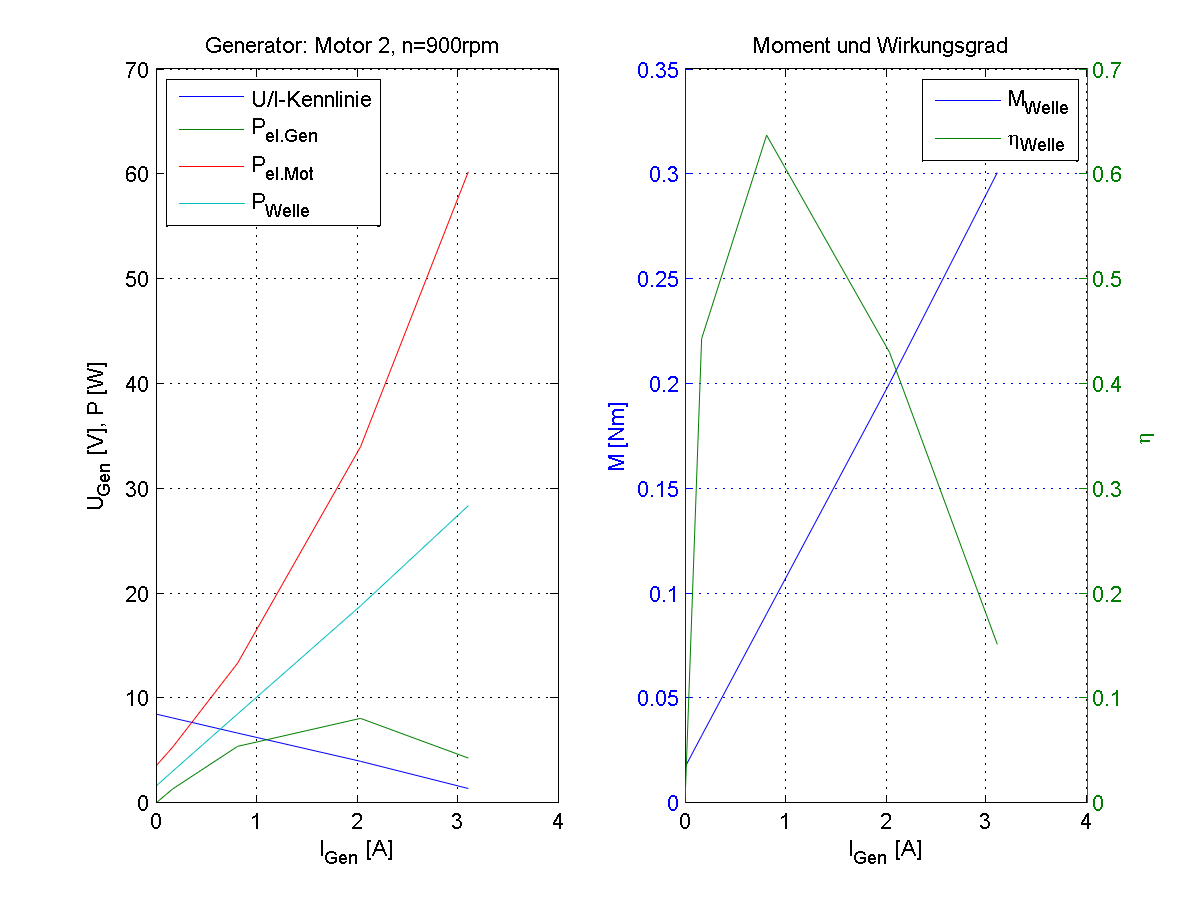
\includegraphics[width=0.49\textwidth]{../plots/aufgabe5-motor1-900rpm.png}}\hfill
	\subfigure[n = 1800rpm]{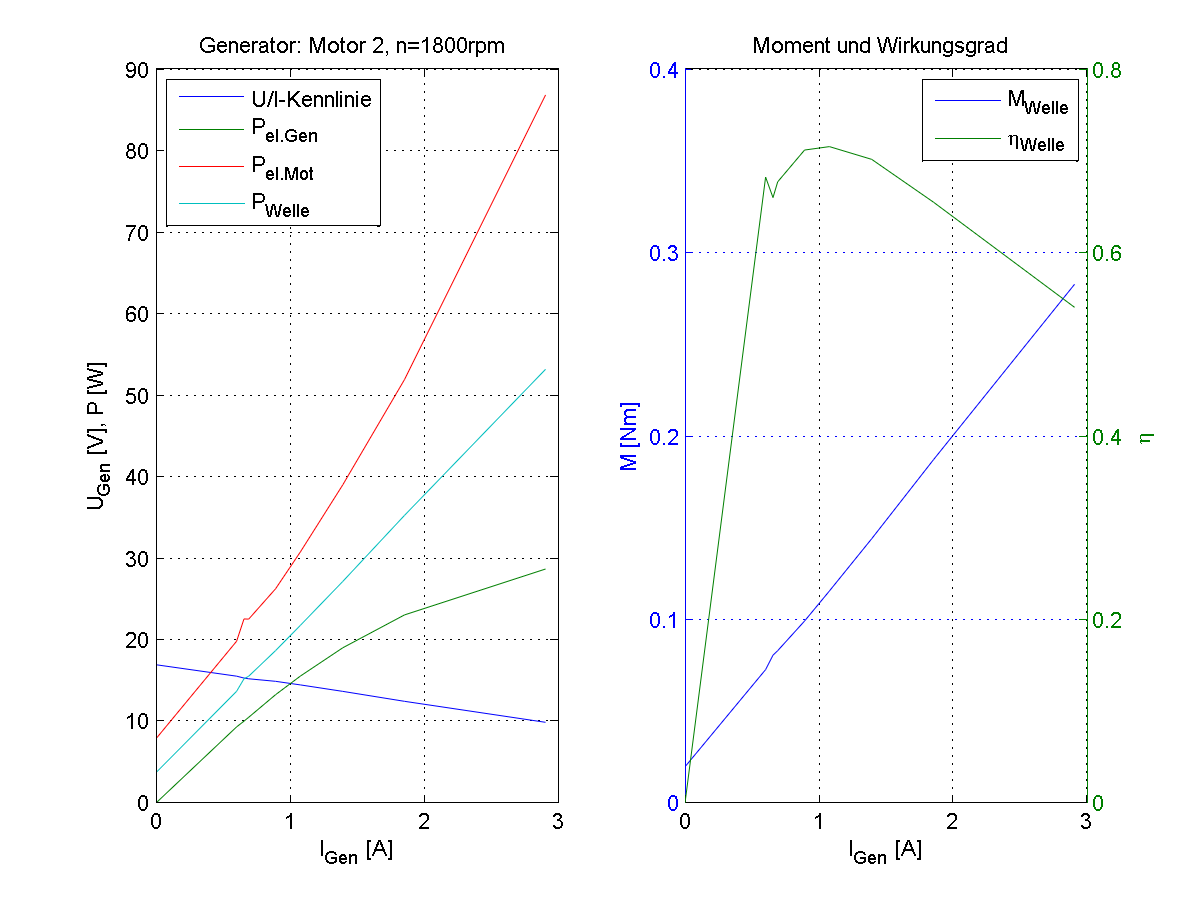
\includegraphics[width=0.49\textwidth]{../plots/aufgabe5-motor1-1800rpm.png}}
	\caption{Motor 1}
	\label{fig:A5_M1_900rpm}
\end{figure}

\begin{figure}[ht]
	\subfigure[n = 900rpm]{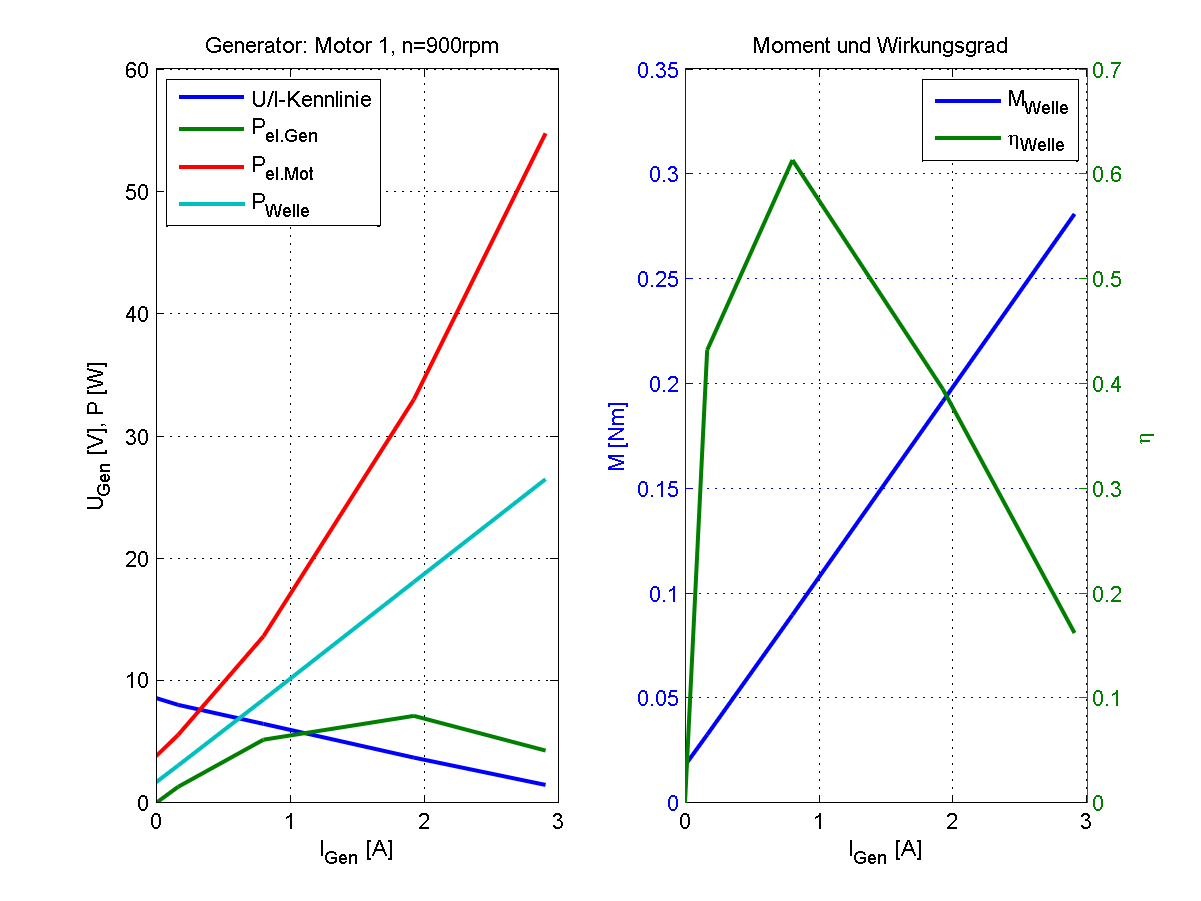
\includegraphics[width=0.49\textwidth]{../plots/aufgabe5-motor2-900rpm.png}}\hfill
	\subfigure[n = 1800rpm]{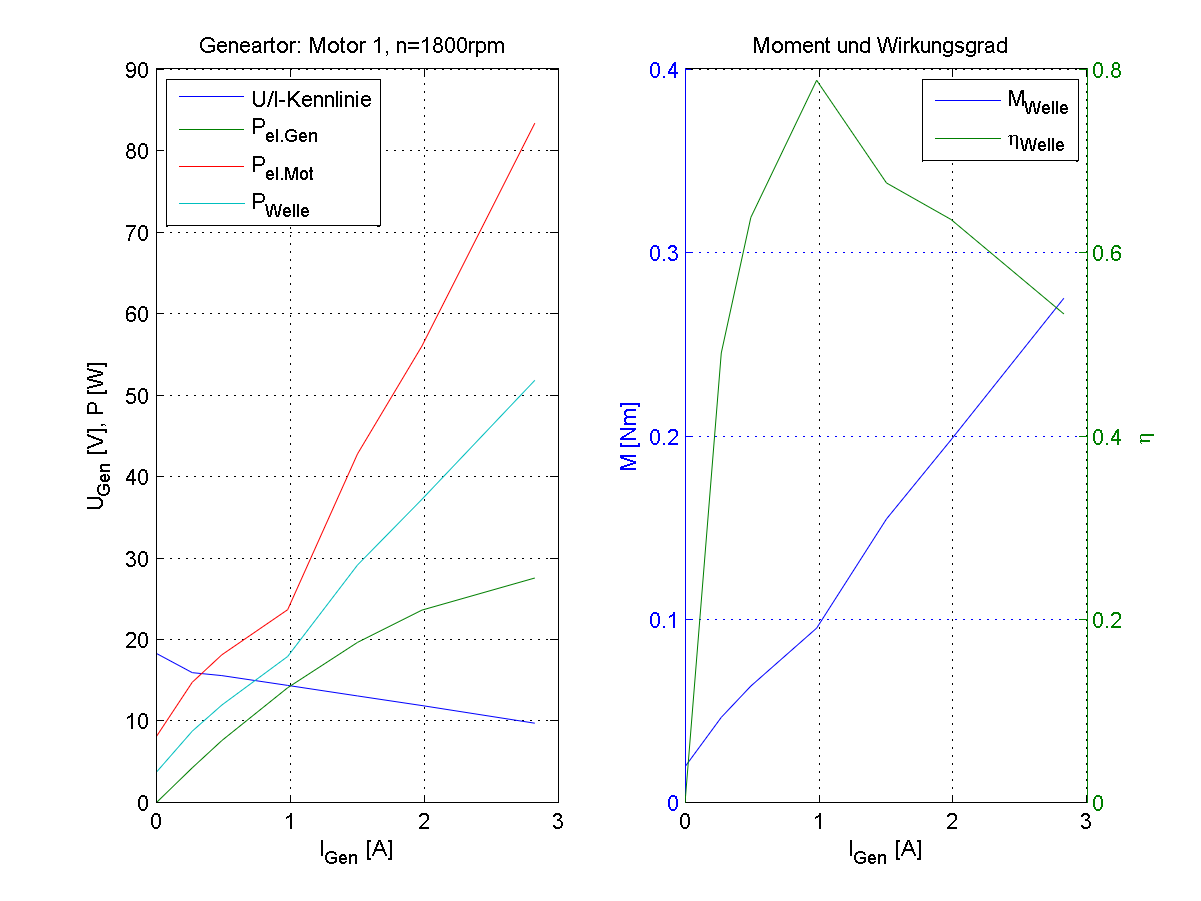
\includegraphics[width=0.49\textwidth]{../plots/aufgabe5-motor2-1800rpm.png}}
	\caption{Motor 2}
	\label{fig:A5_M2_900rpm}
\end{figure}
\subsection{Aufgabe 6}
F�r die Berechnung von $n$ in Abh�ngigkeit des inneren Momentes wurde Gleichung \ref{eq:n-mi} verwendet:

\begin{equation}
n = \frac{U_A}{c \cdot \Phi} \mp \frac{2 \cdot \pi \cdot R_A}{(c \cdot \Phi)^2}  \cdot  M_i \mp \frac{2 \cdot U_B}{c \cdot \Phi}
\label{eq:n-mi}
\end{equation}

Da $M_i$ nicht direkt bekannt ist, wurde Gleichung \ref{eq:mi} angewendet, um vom Strom $I_{Gen}$ auf das innere Moment zu kommen:

\begin{equation}
M_i = \frac{c}{2 \pi} \cdot \Phi \cdot I_A
\label{eq:mi}
\end{equation}

Die Resultate dieser Berechnung sind in den Diagrammen von Aufgabe 7 (siehe \autoref{sec:aufgabe7}) enthalten.

\subsection{Aufgabe 7}
\label{sec:aufgabe7}

Das Moment $M_{Welle}$ wurde nach Gleichung \ref{eq:mwelle} berechnet:

\begin{equation}
M_{Welle} = \frac{1}{2} \cdot \left( \frac{c_{Mot} \cdot \Phi_{Mot}}{2 \pi} \cdot I_{AMot} + \frac{c_{Gen} \cdot \Phi_{Gen}}{2 \pi} \cdot I_{AGen} \right)
\label{eq:mwelle}
\end{equation}

Da aber laut \autoref{tab:cphi} $c_{Mot} \cdot \Phi_{Mot} = c_{Gen} \cdot \Phi_{Gen}$, kann diese Gleichung noch vereinfacht werden:

\begin{equation}
M_{Welle} = trololo
\label{eq:mwelle2}
\end{equation}


\section{Schlussfolgerung}

\section{Unterschriften}

\vfill
\begin{tabular}{rr}
	\\
	\\
	\\
	\\
	\toprule
	\scriptsize{Datum und Unterschrift}	\hspace{3cm}	&	\textsc{Marcel B�rtschi}	\\
	\\
	\\
	\\
	\\
	\toprule
	\scriptsize{Datum und Unterschrift}	\hspace{3cm}	&	\textsc{Cyril Stoller}
\end{tabular}


% Der Anhang kommt auf eine neue Zeile
\newpage
% Offizielle "A Anhang" Aufz�hlungsvariante
\appendix
% Nur im Inhaltsverzeichnis hinzuf�gen (mit richtiger Seite, da vorher "\newpage"), aber kein Text
\addcontentsline{toc}{section}{Anhang}

% Quellenverzeichnis
%\addcontentsline{toc}{section}{Quellenverzeichnis}
\section{Quellenverzeichnis}
\renewcommand\refname{}

%\vspace{-1cm}

\bibliographystyle{amsplain}
\bibliography{Bildquellen}

\section{Messmittelliste}
\begin{itemize}
	\item Multimeter: 2x TENMA 72-7755
	\item Multimeter: RO-334
	\item Multimeter: Siemens Multizet (MM 602-1)
	\item Speiseger�t: Kepco (MN 605-5)
	\item Speiseger�t: Delta SM 7020-D (MN 604-1)
	\item Motor: LM2008-2
	\item Lastwiderstand $18\Omega$
	\item Lastwiderstand $46\Omega$
\end{itemize}

\section{Matlab Code}
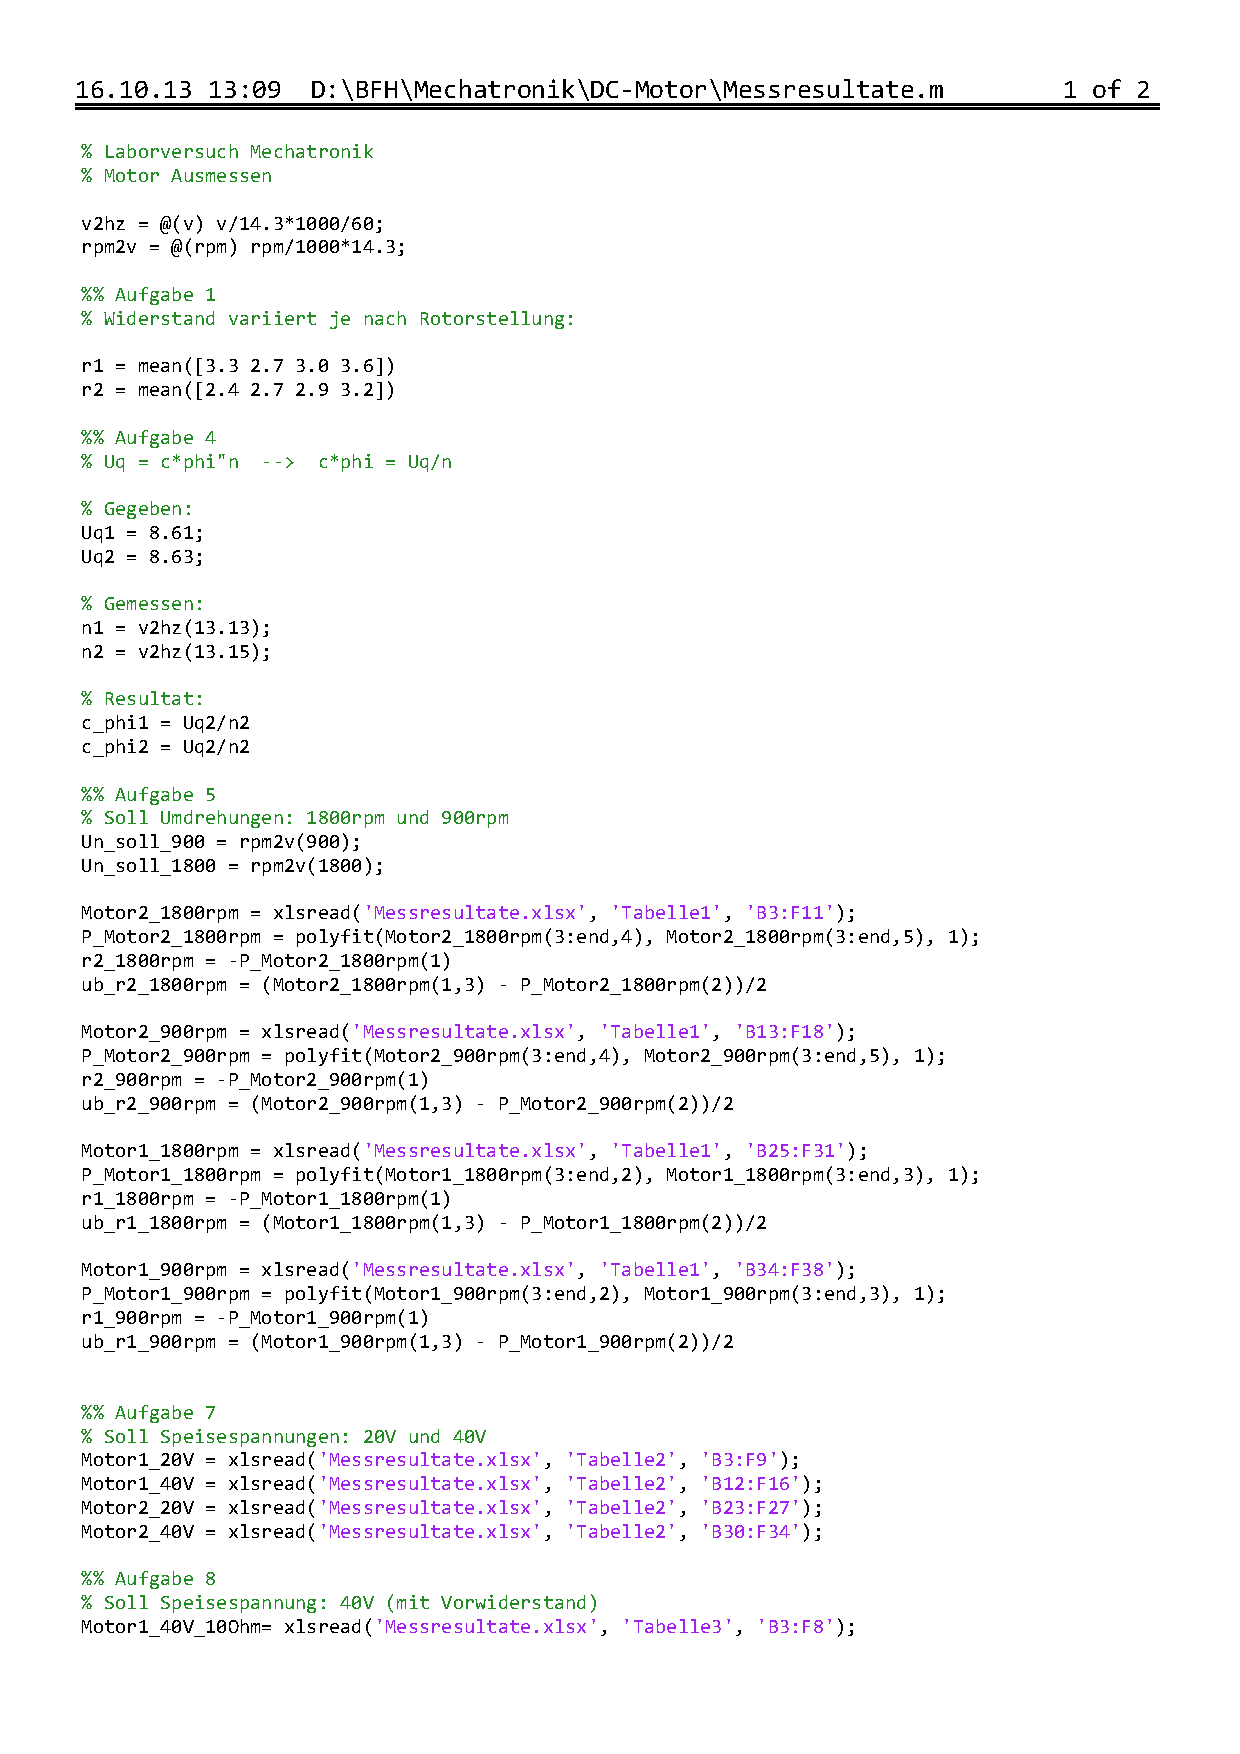
\includepdf{Matlab-Skript.pdf}

\section{Aufgabenstellung Praktikum}
\label{sec:aufgabe}
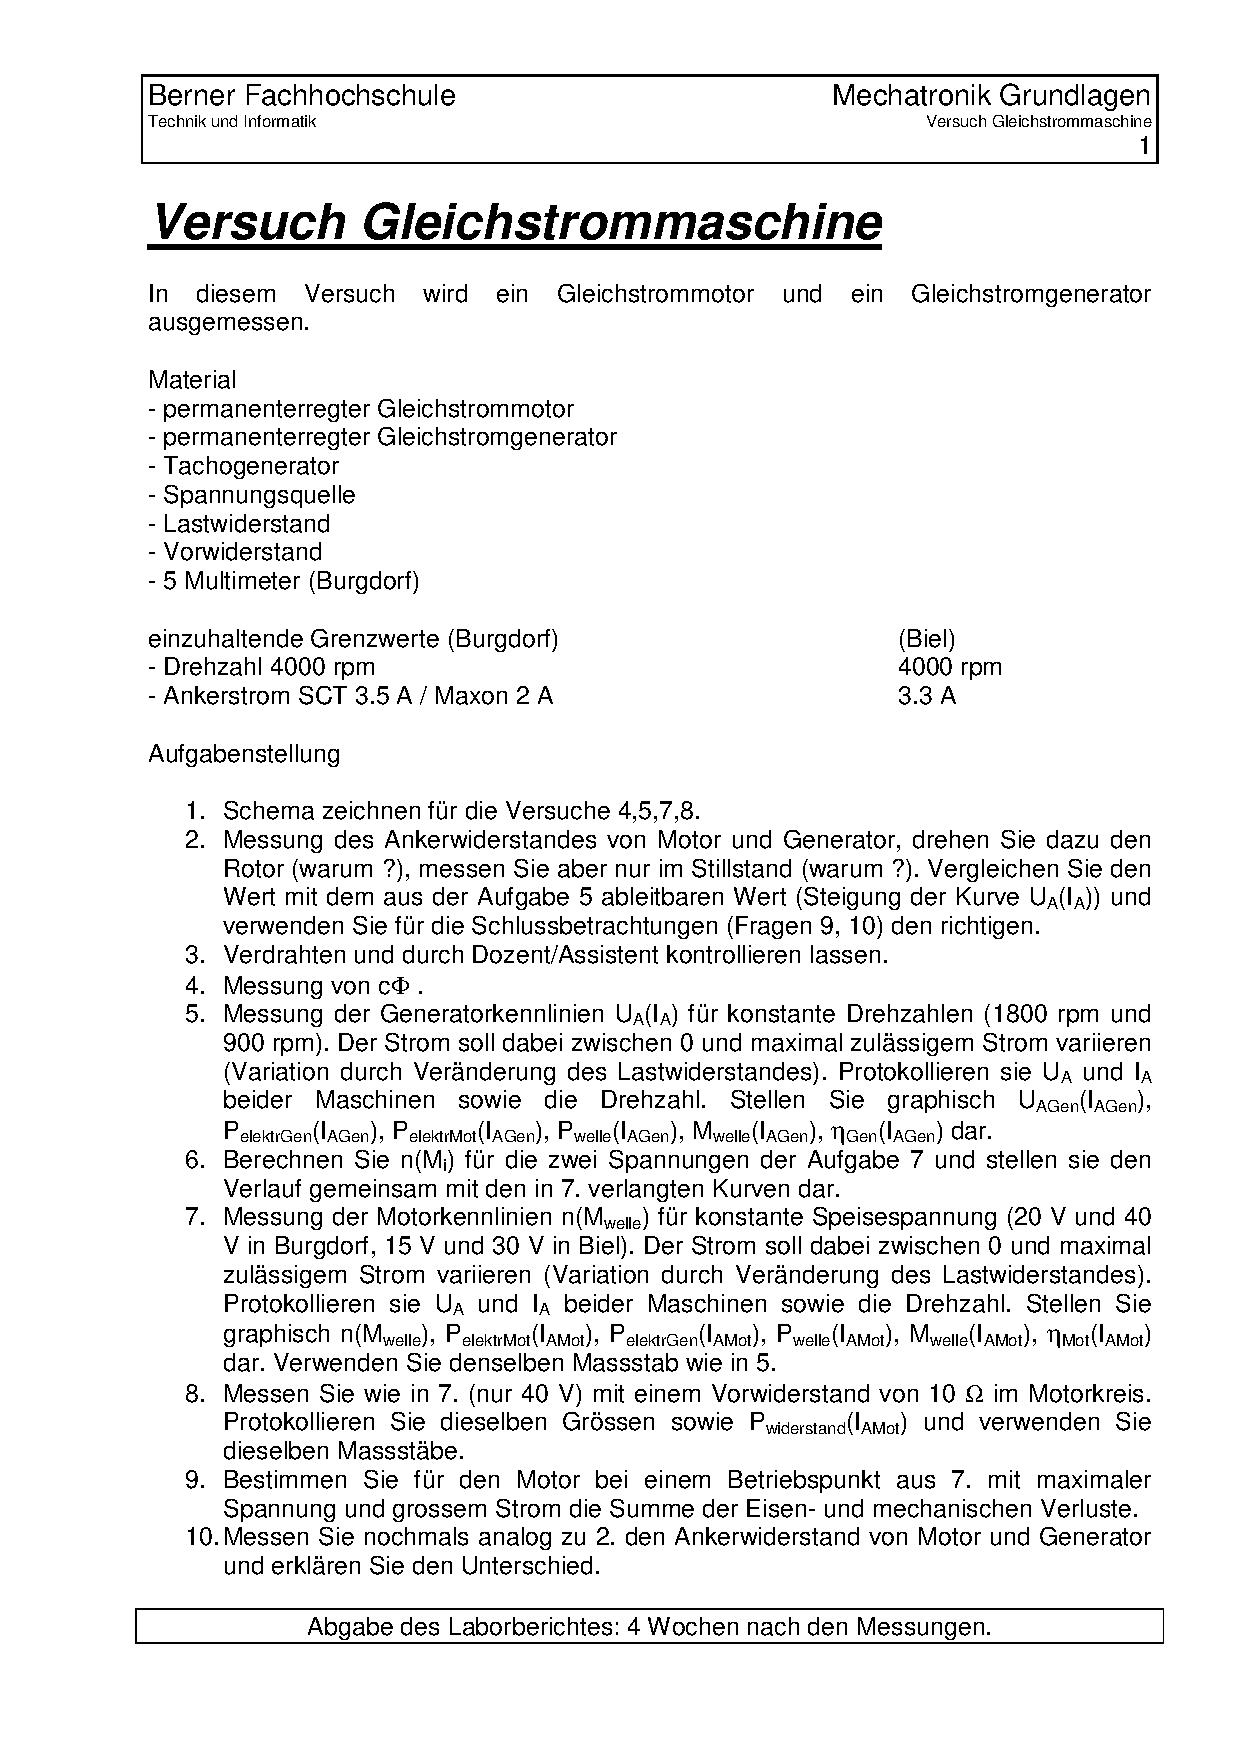
\includepdf{Anhang-Versuch-Gleichstrommaschine.pdf}

\end{document}
